%%%%%%%%%%%%%%%%%%%%%%%%%%  phdsymp_sample2e.tex %%%%%%%%%%%%%%%%%%%%%%%%%%%%%%
%% changes for phdsymp.cls marked with !PN
%% except all occ. of phdsymp.sty changed phdsymp.cls
%%%%%%%%%%                                                       %%%%%%%%%%%%%
%%%%%%%%%%    More information: see the header of phdsymp.cls   %%%%%%%%%%%%%
%%%%%%%%%%                                                       %%%%%%%%%%%%%
%%%%%%%%%%%%%%%%%%%%%%%%%%%%%%%%%%%%%%%%%%%%%%%%%%%%%%%%%%%%%%%%%%%%%%%%%%%%%%%


%\documentclass[10pt]{phdsymp} %!PN
\documentclass[twocolumn]{phdsymp} %!PN
%\documentclass[12pt,draft]{phdsymp} %!PN
%\documentstyle[twocolumn]{phdsymp}
%\documentstyle[12pt,twoside,draft]{phdsymp}
%\documentstyle[9pt,twocolumn,technote,twoside]{phdsymp}

\usepackage[english]{babel}       % Voor nederlandstalige hyphenatie (woordsplitsing)

\usepackage{graphicx}                   % Om figuren te kunnen verwerken
\usepackage{graphics}			% Om figuren te verwerken.
\graphicspath{{fig/}}               % De plaats waar latex zijn figuren gaat halen.

\usepackage{times}

\hyphenation{}

\def\BibTeX{{\rm B\kern-.05em{\sc i\kern-.025em b}\kern-.08em
    T\kern-.1667em\lower.7ex\hbox{E}\kern-.125emX}}

\newtheorem{theorem}{Theorem}

\begin{document}

\title{Een privacyvriendelijk aanbevelingssysteem\\ voor mobiele toestellen} %!PN

\author{Thorwald Frederik Lambrecht}

\supervisor{Marleen Denert, Luc Martens, Toon De Pessemier}

\maketitle

\begin{abstract}
Dit artikel probeert het ideale privacyvriendelijke aanbevelingssysteem te cre\"eren voor een mobiel toestel. In dit proces zal het trachten de grenzen van de wisselwerking tussen privacy, nauwkeurigheid en performantie bij aanbevelingssystemen te verleggen. Om dit te bereiken wordt een methode gebruikt op basis van homomorfische encryptie.
\end{abstract}

\begin{keywords}
Privacy, mobiel, aanbevelingssysteem
\end{keywords}

\section{Inleiding}
\PARstart{O}{m} gepersonaliseerde aanbevelingen toe te laten hebben aanbevelingssystemen privacygevoelige data nodig van hun gebruikers. Dit verplicht de \emph{service provider} om deze data bij te houden en 
opent de poort voor de privacy inbreuken. Deze inbreuken kunnen het gevolg zijn van een oneerlijke provider of een na\"ieve gebruiker, maar ook van onvoldoende data bescherming tegenover aanvallen.\\ Er bestaan verschillende benaderingen om de privacy van de gebruiker te verbeteren. Eerst en vooral kan de gebruiker beter ingelicht worden over de grootteorde waarop zijn data wordt bijgehouden en de wijze waarop ze gebruikt wordt. Ten tweede zou de wet rond privacy strikter kunnen gemaakt worden. Een andere mogelijkheid is het gebruik van privacyvriendelijke algoritmes.\\
Het gebruik van bestaande algoritmes vermindert minstens de nauwkeurigheid van de aanbevelingen of de performantie. Rekening houdend met de mobiele setting, is het ook belangrijk om een werkwijze te vinden die niet veel processortijd of data overdracht nodig heeft op de client. Om uit te zoeken hoe een aanbevelingssysteem in een mobiele setting de wisselwerking best aanpakt, was er onderzoek nodig in de bestaande privacyvriendelijke oplossingen.

\section{Onderzoek naar bestaande privacyvriendelijke methodes}
Er bestaan verschillende methodes om de privacy te verbeteren in aanbevelingssystemen. Deze methodes omvatten werkwijzes met behulp van anonimisatie, randomisatie, aggregatie van gebruikersprofielen en cryptografische protocollen. Voor elk van deze mogelijkheden werd er een grondige analyse gedaan van minstens \'e\'en voorbeeldoplossing en werd er een vergelijking gemaakt. \\ De oplossing gebaseerd op anonimisatie \cite{anonimisatie} maakt gebruik van agents die anoniem communiceren met elkaar. Ondanks het feit dat gedurende de aanvragen en de vergelijking van gebruikers onderling voor user-user collaborative filtering, de gebruikers anoniem blijven, garandeert anonimiteit geen privacy. Dit is bewezen door Narayan \cite{anon}.\\Het randomisatie algoritme gebruikt door Polat en Du \cite{rand} voorziet ook niet in volledige privacy voor de gebruiker, aangezien de server nog steeds de range van waarden weet waartussen een gebruiker zijn aparte waarden liggen. De methode verliest ook sterk aan nauwkeurigheid bij het gebruik van kleine datasets.\\  Het gebruik van aggregatie van gebruikersprofielen door Shokri et al. in \cite{agg} biedt de gebruiker de mogelijkheid om zijn voorkeuren te ontkennen maar toont de server nog steeds originele beoordelingen van de gebruiker. Deze werkwijze verliest boet wel niet aan nauwkeurigheid in. \\ De oplossing aan de hand van cryptografische protocollen met gebruik van een peer-to-peer  relatie tussen clients \cite{social} is wel privacyvriendelijk maar heeft een sociaal netwerk nodig waar gebruikers vaak online zijn. De methode vraagt ook te veel berekeningen aan de clientkant voor een mobiele setting.\\ De beste methode lijkt deze op basis van cryptografische protocollen met twee servers door Erkin et al \cite{dyn}. Deze aanpak gebaseerd op een eerdere oplossing \cite{erkin} biedt een hoog privacyniveau en vereist geen zware berekeningen aan de clientkant. Op basis van deze vaststelling werden de cryptografische protocollen van deze methode gekozen om te dienen als basis voor deze oplossing.

\section{De privacyvriendelijke oplossing}
We besloten om een native androidapplicatie te maken en de servers werden geschreven in Java. Ze communiceren allemaal onderling met het HTTP-protocol. Als testdatabank werd de MovieLens databank gebruikt met 100.000 beoordelingen, 943 personen en 1682 films. De oplossing in \cite{dyn} maakt gebruik van twee servers, een aanbevelingsserver en een tweede server die wordt ingezet door een betrouwbare derde partij. De clientapplicatie stuurt de beoordelingen en voorkeuren van de gebruikers naar de aanbevelingsserver, ze zijn ge\"encrypteerd met de publieke Pailliersleutel van de tweede server. Dit hoeft niet elke keer te gebeuren als een gebruiker een item beoordeelt. Om een voorspelling te doen van een beoordelingswaarde voor een item is er communicatieprotocol nodig tussen de twee servers op basis van hun Paillier en DGK cryptosysteem. Dit protocol telt het aantal en de som van de ge\"encrypteerde ratings van gebruikers met gelijkaardige voorkeuren.



 To generate a prediction score for an item communication is needed between the Paillier and DGK cryptosystems on both servers to sum and count the encrypted ratings of like-minded users. The like-minded users are calculated by the known Pearson-correlation, which is partly computated by the client. For the computations on the serverside for the Pearson-correlation it uses complicated protocols between the two servers like a multiplicationprotocol and a thresholdprotocol. There are several practical decisions that needed to be taken when implementing these protocols, especially on the userside. As opposed to \cite{dyn} the user should not send his encrypted ratings individually. This would enable the recommenderserver to know he just rated an item. An option is to choose several random items and include encrypted zero-values for these. However the items could randomly all be chosen in a particular field and thus giving the service provider information. This could be avoided by choosing these items in a smart way, but this leaves values like his preferences and offsets calculated by an old mean. To have optimal privacy in our application the user sends his ratings and preferences, also called his profile, in one time, with encrypted zero values for all items that aren't rated. For this solution it is necessary that per rating there is another bit encrypted by the user added to his profile. This encrypted bit $ q_{U_x,i} $ that is 1 if the user x has rated the item i and 0 if not. This makes it possible to count the number of effectively rated items used in our formula (\ref{stdrecom}). The encryption of the values is also best calculated the moment the user sends his profile. Otherwise the server could see which encrypted values are changed. In the original paper \cite{dyn} calculates a prediction by taking the average value of the ratings for that item from users that score a similarityvalue above a thresholdvalue. However the protocols used allow an improvement by generating predictions based on a version of a formula used often in user-user collaborative filtering:
\begin{equation}\label{stdrecom}p_{U_1,i} = \bar{r}_{U_1} + \frac{\sum_{j=2}^{n}(r_{(U_j,i)} - \bar{r}_{U_j}).s_{(U_1,U_j)}.q_{(U_j,i)}}{\sum_{j=2}^{n} s_{(U_1,U_j)}.q_{(U_j,i)} }
\end{equation}
where $r_{(U_x,i)}$ denotes the rating value for user x for item i, $\bar{r}_{U_x}$ the average over all items for user x and $p_{U_1,i}$ denotes the prediction from user 1 for item i.
Here the value $s_{(U_1,U_j)}$ stands for the bit that is calculated by the thesholdprotocol and this bit is 1 if the user has a similarity above the thresholdvalue. In stead of the ratingvalue itself, the user now sends the encrypted offset from his average $\bar{r}_{U_1}$. This value has to be converted to a positive integer for the use of the cryptosystems. This can happen in an easy way $result = ((r_{(U_j,i)} - \bar{r}_{U_j})+5)*1000$. Once the sum is taken over all the similar users, the client can revert the conversion by division through 1000 and subtracting 5 per similar user.

\section{Results}
The predictions of the improved method (the light line)  shows significant better scores for accuracy than the method from \cite{dyn} (the dark line). 

\begin{figure}[ht]
\begin{center}
	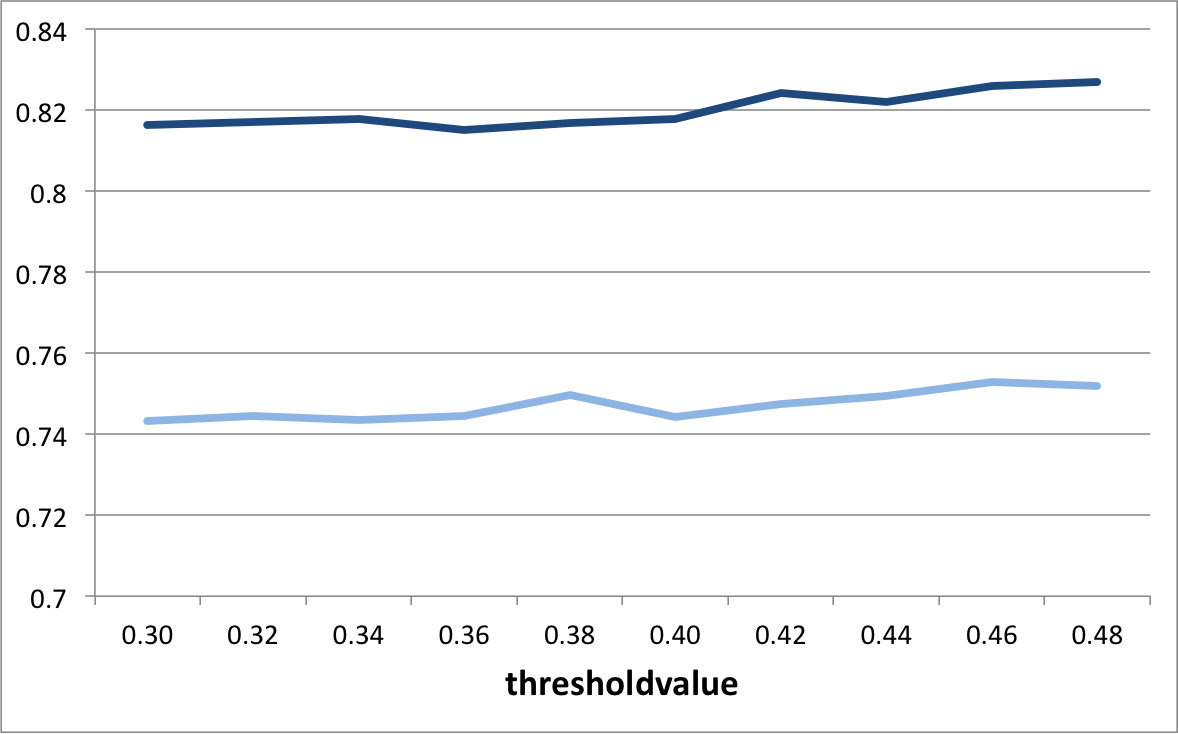
\includegraphics[width=.40\textwidth]{mae}
	\caption{MAE results over 10.000 predictions over different thresholdvalues}
\end{center}
\end{figure}
\begin{figure}[ht]
\begin{center}
	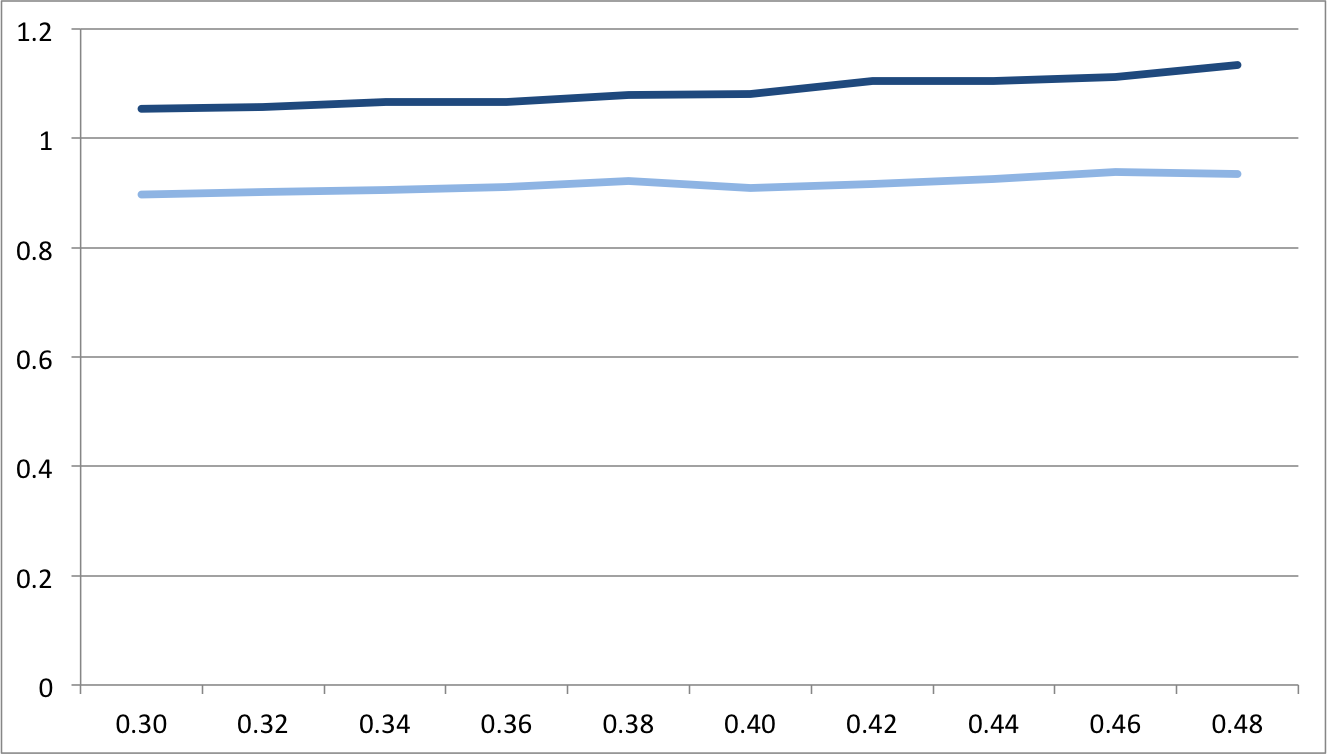
\includegraphics[width=.40\textwidth]{mse}
	\caption{MSE results over 10.000 predictions over different thresholdvalues}
\end{center}
\end{figure}

The MAE improved from around 0.82 to around 0.74, this is very close to the MAE of a privacy-unfriendly solution on the same database by \cite{rand} which is 0.7146. Since the privacy is unchanged our solution still obtains very high privacy levels. The performance on our mobile device is $O(N+S)$ with N as number of items and S as number of preferences. This contains the encryption of a userprofile and thus for each item 2 encryptions and for each preference 1 encryption was done by our testtablet \footnote{Samsung Galaxy Tab4 (7.0) Wi-Fi on Android 4.4.2} in 1,52 seconds averaged over 10 times. The servers engage in heavy computation, it took our testserver\footnote{MacBook Pro 4 GB RAM 2.4 GHZ i7 processor} 7 minutes 26 seconds to generate predictions for all 1682 items for one user, when using 30 preferences. This however can still be optimized with the use of a lower-level protocol as it was, looking back, not the best choice of using the HTTP-protocol for the communication between the two servers. Also the user could send less values to the server at once as discussed. This would have an impact on the accuracy of the algorithm but would decrease the work at the serverside and the size of its' database.

 
\section{Conclusion}

The solution provided guarantees a very high level of privacy by the use of encryption with Paillier and DGK and the fact that the server does not know which items are rated by the user. It also offers high accuracy scores without a lot of computation on the clientside. These properties make it ideal for use as a recommender for mobile devices. The servers themselves have to engage in heavy computation but this computation could be further optimized.








\nocite{*}
\bibliographystyle{phdsymp}
%%%%%\bibliography{bib-file}  % commented if *.bbl file included, as
%%%%%see below


%%%%%%%%%%%%%%%%% BIBLIOGRAPHY IN THE LaTeX file !!!!! %%%%%%%%%%%%%%%%%%%%%%%%
%% This is nothing else than the phdsymp_sample2e.bbl file that you would%%
%% obtain with BibTeX: you do not need to send around the *.bbl file        
%%
%%---------------------------------------------------------------------------%%
%
\begin{thebibliography}{1}
\bibitem{anonimisatie}

Ciss{\'e}e, Richard and Albayrak, Sahin
\newblock {\em An Agent-based Approach for Privacy-preserving Recommender Systems},
\newblock Proceedings of the 6th International Joint Conference on Autonomous Agents and Multiagent Systems,2007

\bibitem{anon}
Narayanan, Arvind and Shmatikov, Vitaly
\newblock{\em Robust De-anonymization of Large Sparse Datasets},
\newblock Proceedings of the 2008 IEEE Symposium on Security and Privacy, 2008

\bibitem{rand}
Polat, Huseyin and Du, Wenliang
\newblock{\em SVD-based Collaborative Filtering with Privacy},
\newblock Proceedings of the 2005 ACM Symposium on Applied Computing,2005


\bibitem{agg}
Shokri, Reza and Pedarsani, Pedram and Theodorakopoulos, George and Hubaux, Jean-Pierre
\newblock{\em Preserving {P}rivacy in {C}ollaborative {F}iltering
                 through {D}istributed {A}ggregation of {O}ffline
                 {P}rofiles},
\newblock{The 3rd {ACM} {C}onference on {R}ecommender {S}ystems ({R}ec{S}ys), 2009}

\bibitem{dyn}
Zekeriya Erkin and Thijs Veugen and R.L. Lagendijk
\newblock{\em Privacy-Preserving Recommender Systems in Dynamic Environments},
\newblock IEEE Workshop on Information Forensics and Security, 2013

\bibitem{erkin}
Zekeriya Erkin and Michael Beye and Thijs Veugen and Reginald L. Lagendijk
\newblock{\em Efficiently computing private recommendations},
\newblock ICASSP,2011


\bibitem{social}
Hoens, T. Ryan and Blanton, Marina and Chawla, Nitesh V.
\newblock{\em A Private and Reliable Recommendation System for Social Networks},
\newblock{Proceedings of the 2010 IEEE Second International Conference on Social Computing, 2010}

\end{thebibliography}
%
%%---------------------------------------------------------------------------%%

\end{document}

%%%%%%%%%%%%%%%%%%%%%  End of phdsymp_sample2e.tex  %%%%%%%%%%%%%%%%%%%%%%%%%%%
